\chapter{Background and Approach}
\label{background}

This chapter examines ICT-supported citizen participation in crisis events (specifically the phenomenon known as digital volunteerism) and how it relates to the problem of pet-to-family reunification in disaster.  In addition, this chapter discusses the need for computational support of volunteers' activities in the form of machine learning and examines literature that has influenced my design of this system.

\section {Pets in Crisis Situations}

Though exact figures are difficult to obtain, it is estimated that 50 to 70 percent of American households (approximately 61 to 86 million) include at least one pet.  When disaster strikes, pets are often left behind in evacuations because they cannot be transported or allowed into shelters.  In the case of large-scale disasters, the displacement of pets creates a variety of serious problems.  During Hurricane Katrina, an estimated 200,000 pets were displaced from their guardians; only five percent of these pets were ever reunited with their guardians \cite{lowe:petloss}.  Many displaced pets were disposed of or ``rehomed'' to families in other states, which in some cases even resulted in legal disputes over pet ownership when the original guardians of a pet located it \cite{mcnabb:courts}.  

Animals displaced by disaster can create large public health hazards.  In addition, displaced or abandoned pets can be the source of public safety issues as evacuated disaster victims will return to hazardous areas in order to retrieve them.  The challenges of incorporating pets into disaster planning were recognized by the federal government's passing of The Pets Evacuation and Transportation Standards (PETS) Act of 2006 in response to challenges faced during Hurricane Katrina and its aftermath.  

Furthermore, disaster victims who leave pets behind may be ill-suited to attempt to locate them remotely; in the aftermath of a disaster, victims (especially those residing at a temporary shelter) may have limited access to communications technology such as phones or computers.  This was seen in the conditions of Hurricane Katrina victims who were located at shelters - these residents had extremely limited access to land line phones and although some residents had cell phones, coverage was limited and charging them was a challenge \cite{palen:ict}.  It is also unrealistic to expect disaster victims to spend what little time they have with ICT in the aftermath of a disaster searching for lost pets.  Finally, a single person may be unable to adequately search for a given pet in a potentially vast search space.  For example, if even ten percent of lost and found pets in Hurricane Katrina were reported digitally, an individual would need to search through approximately 20,000 pet reports to find a single animal.  Directing the efforts of the crowd (in the sense of crowd work) can mitigate this problem by increasing collaboration and distributing work.  

\section {Digital Volunteerism}

An interesting development in the field of crisis informatics has been the study of digital volunteerism.  Digital volunteerism \cite{starbird:voluntweeters} is a technological expansion of traditional volunteer activities that occur in disaster situations \cite{fritz:convergence, palen:ict}, and is characterized by improvisation and self-organization by the people involved in volunteer activities.  Digital volunteers are defined by their location, as they are usually volunteers who are geographically removed from a disaster but still want to be involved in volunteer efforts via online activity.

Starbird and Palen explored digital volunteerism in the aftermath of the 2010 Haiti earthquake as remote volunteers converged through Twitter to process information and make connections between requests for help and offers of assistance \cite{starbird:voluntweeters}.  Self-named ``voluntweeters'', these digital volunteers primarily engaged translating crisis tweets from their original format into the ``Tweak the Tweet'' syntax \cite{starbird:ttt}, which is machine readable, effectively synthesizing unstructured information (from multiple sources) into structured, usable data.  Many interviewed volunteers engaged in auxiliary tasks in addition to the core translation activity, such as {\em verifying} the content of a tweet or acting as a remote operator by {\em routing} information \cite{starbird:voluntweeters}.  It is important to note that the volunteers in this study performing these more complex tasks were unable to use the core social media platform (Twitter) to perform the entirety of their work; this suggests that there is space for specialized tools to be built that leverage social media but accommodate the needs of digital volunteers.

Specialized tools can not only accommodate the needs of digital volunteers but also deal with issues of information convergence that arise when dealing with crowd work in the crisis space.  Starbird identifies these issues \cite{starbird:doctoral} as:

\begin{itemize}
  \item{} {\em Noisy information space}: the information space of a social media platform such as Twitter, even when filtered through the use of mechanisms such as hashtags, is still noisy and must be filtered further so that relevant information can be identified.
  \item{} {\em Loss of context}: information which is routed through social media is subject to modification by the users performing the routing mechanism (in the case of Twitter, this often takes the form of the retweet mechanism).  Modification of information and even the simple act of information passing can cause loss of contextual information.
  \item{} {\em Misinformation and disinformation}: incorrect information can hinder the activities of digital volunteers and even be dangerous in a disaster situation; information must therefore be subject to a verification mechanism.
  \item{} {\em Organization and data structure}: to be more useful, information needs to be compatible with computational resources, such as search engines and databases.  Information must therefore be structured in a systematic manner.
\end{itemize}

The use of specialized tools in the disaster space can alleviate these issues in a variety of ways.  First, specialized tools will most likely impose some structure on the the specific data being used within a system; this immediately addresses the problem of organization and data structure of information.  Furthermore, because a specialized tool is not limited by structural limitations on data format present in some major social media platforms (such as Twitter), it can more effectively address the problem of loss of context.  For example, retweeted information on Twitter may lose contextual information due to user modification or simple loss of textual content stemming from the 140-character limit on tweet size.  A specialized tool might overcome this limitation by storing more detailed history of a particular information item, thereby preserving the various contexts associated with that item.  Finally, a specialized tool can integrate computational and social solutions to address the problems of noisy information and misinformation, which might include, for example, an information retrieval system catered to the data structures managed by the tool to alleviate noise and including a voting mechanism to mitigate misinformation.

\section {The Data Scouts Framework}

The goal of the Data Scouts framework \cite{sdc, palen:proposal} is to classify the digital volunteer into one of three roles: the {\em data scout}, {\em consolidator}, or {\em checker}.  The characteristics of these roles are briefly described in Figure~\ref{fig:datascouts}.

\begin{figure}[htbp]
    \begin{center}
	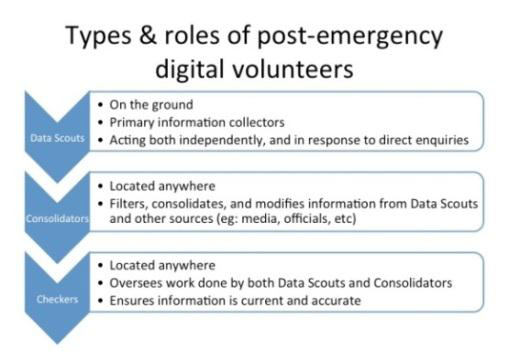
\includegraphics[width=90mm]{figs/datascouts.png}
    \end{center}
        \caption[Data Scouts Roles]{
        The three types of digital volunteer activity in the Data Scouts framework
	}
	 \label{fig:datascouts}
\end{figure}

This framework introduces a new category of volunteer, the data scout, whose role is to provide on-the-ground data for use by remote digital volunteers.  In the domain of pets in disaster, the data scout is the volunteer who is at a shelter reporting animals that reside there, or just an individual who has lost or found a pet during the disaster.

The importance of this framework with regard to this work is that it classifies the behaviors of digital volunteers discussed previously into specific roles.  Consolidators engage in synthesis tasks like information translation and routing; checkers engage in the important task of information verification.  It is important to note that the roles delineated by this framework are not by any means mutually exclusive; it is highly likely that digital volunteers might take on one or more roles during a crisis event.  Nevertheless, the roles that this framework provides are highly useful because we can use them as a starting point for system design.  The system described in this work makes heavy use of the roles described here.

\section {Machine Learning to Support Human Activity}

Machine learning is often thought of as being orthogonal to human computation, but there are many machine learning approaches and paradigms that view human computation as complementary to machine computation; this work embraces this view.  The idea that human and machine computation are at their best when placed in complementary roles is not a new one; in 1960, J. R. Licklider envisioned the future of computing as one where man and machine acted in symbiosis, with computers acting as colleagues to their human counterparts \cite{licklider:symbiosis}.  This vision is reflected in many machine learning systems today, such as recommendation systems and autonomous agents.

The study of autonomous agents has a heavy influence on the design of the machine learning components presented in this work.  Autonomous agents encompass a variety of artificial intelligence techniques and have a somewhat controversial definition \cite{franklin:taxonomy}, but the essential idea is one of a learning software system which acts in collaboration with a human user.  Such a system necessarily is viewed as an assistant to the user, and this assistant is generally expected to become more proficient over time at whatever tasks it is delegated.  Agents can assist users in a wide variety of ways, ranging from performing complex computation, training users, performing tasks on behalf of users, or even helping multiple human users collaborate \cite{lieberman:agents, maes:agents}.  As such, the set of problem domains in which they are applicable is large and includes information filtering and retrieval, which is the core task of the machine learning component presented in this work.

A key aspect of autonomous agents is that in collaborating with users, they are not the primary authoritative actor that makes decisions.  Agents may perform tasks on behalf of users or recommend courses of action, but they do not prohibit users from taking independent action.  This quality helps mitigate the imperfect nature of artificially intelligent systems and can focus the design of machine learning systems onto tasks which are ideally suited to their use.

Placing machine computation in the role of a collaborator instead of a complete solution to problems is a view that meshes well with many problems in crisis informatics.  Machine learning can play a large role in crisis informatics technology, especially in information retrieval and extraction.  For example, natural language processing and classification techniques have been shown to be effective in deciding whether or not a tweet contributes to {\em situational awareness} in disaster \cite{verma:nlp}.  At the same time, past research details the unique challenges of applying machine learning algorithms to the types of information common in the crisis space \cite{corvey:nlp, starbird:voluntweeters}.  Because we cannot expect machine learning to be a silver bullet solution, especially in the space of crisis informatics, this work takes the approach of implementing machine learning solutions that solve tasks unsuited for human computation.  Furthermore, the machine learning components are designed from an agential paradigm and take opportunities to learn from human computation to better assist human activity.

\section {Envisioning a System for Pet-to-family Reunification}

The problem of pet-to-family reunification is an ideal context in which to build a system which utilizes digital volunteers and combines human and machine computation.  As this chapter has discussed, pet owners who lose their pets may be ill-suited to finding them on their own.  By utilizing digital volunteers (as defined by the Data Scouts framework), we can focus the efforts of an enthusiastic user population on a task that is an important societal problem.  This section examines some of the challenges faced in pet-to-family reunification and discusses how these challenges inform the design of a system, for use by digital volunteers, to solve this problem.

The problem of pet-to-family reunification is complicated because of the fact that pets cannot self-identify after being found in the wake of a disaster by an individual or organization.  Furthermore, the search space of all pets reported lost and found to online services during a disaster is both at once large and sparse --- there may be thousands of reported pets but there is still only a small chance of finding a correct match for any given pet in the space.  Textual profiles of pets generally do not contain sufficient information to be the sole resource used in identifying a pet.  Visual information, such as pictures of a pet, are likely the most valuable identifying information contained in a profile of a lost or found pet.  However, computational techniques for processing this information are likely to be ineffective within the disaster domain.  For example, a pet owner may submit an older photo of a pet when reporting that pet as lost, but a data scout in a shelter may include a photo of that pet in a report that has different visual context, i.e., environment, the age of the pet, the angle of the photograph, the inclusion of other pets in the picture, and other factors.  Nevertheless, I posit that this visual matching task is something that humans, who are highly capable of overcoming challenges like noise and ambiguity, are very much suited to completing.

Using human computation to solve the problem of visual matching is good approach to tackling the problem of pet-to-family reunification, but it does not solve the problems of scale mentioned above.  By designing a software solution around digital volunteerism, we can expand, in a sense, the quantities of human computation available to tackle the problem.  By incorporating social and collaborative features into this solution, we can improve the quality of human computation by providing mechanisms for information routing and verification.  However, even by expanding our user base from pet guardians (searching, in general, for a single lost pet) to cadres of digital volunteers, we cannot expect users to scour over thousands of pet reports.  This is where machine learning systems can play an important role in assisting digital volunteers attempting to reunite lost pets with their guardians.

Although machine learning cannot reliably be used to pick out matches between reports of lost and found pets, if we consider lost and found pets as documents, we might design an information retrieval system to assist volunteers in retrieving what appear to be the most relevant reports for any given pet.  Textual features, as mentioned above, may be insufficient to select a single match out of the entire search space, but it is likely that textual features might be useful in selecting a range of potential matches for consideration by volunteers.  The machine learning component of the system is engaged in information filtering on behalf of digital volunteers.

Furthermore, if we design the machine learning component to take an agential stance, we must look at the activities of digital volunteers (human computation) as opportunities for the machine learning system to improve itself.  This work explores two such training activities: volunteers editing pet reports to improve their usefulness and volunteers proposing and recommending matches between a lost pet report and a found pet report (the fourth chapter presents an evaluation of the effectiveness of this approach in an experimental setting).  By taking this approach, we have proposed a system in which human computation is used to inform machine computation, which in turn provides greater assistance to future human computation.

This chapter has demonstrated that displaced and lost pets in disaster create a variety of health and safety problems to individuals and the public.  This chapter has also examined the phenomenon of digital volunteerism within the context of crisis informatics, as well as the role machine learning systems can play in this space.  The system proposed in this section takes the form of \nplh, an online matchmaking tool which acts as an infrastructure supporting digital volunteers in facilitating pet-to-family reunification.  This system's interface design and conceptual framework was initially explored in Barrenechea et al. \cite{sdc}.  The design and architecture of this system is presented in the following chapter.